\documentclass[aspectratio=169, 10pt]{beamer}

\usepackage{bm} % bold math
\usepackage{fontspec}
\usepackage{minted}
\usepackage{pgf-pie}
\usepackage{tikz}
\usepackage{graphicx}
\newcommand\sbullet[1][.5]{\mathbin{\vcenter{\hbox{\scalebox{#1}{$\bullet$}}}}}

% Custom commands and environments
\makeatletter
\newcommand\version[1]{\renewcommand\@version{#1}}
\newcommand\@version{}
\def\insertversion{\@version}

\newcommand\course[1]{\renewcommand\@course{#1}}
\newcommand\@course{}
\def\insertcourse{\@course}

\newcommand\coursetitle[1]{\renewcommand\@coursetitle{#1}}
\newcommand\@coursetitle{}
\def\insertcoursetitle{\@coursetitle}

\newcommand\lecturenumber[1]{\renewcommand\@lecturenumber{#1}}
\newcommand\@lecturenumber{}
\def\insertlecturenumber{\@lecturenumber}
\makeatother

\newcommand{\slidetitle}[1]{{\xbseries \large \structure{#1}} \bigskip}
\newcommand{\term}[1]{{\color{blue} #1}}
\newcommand{\leftspace}{\hspace{1em}}
\newcommand{\inlinearrow}{
  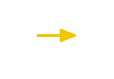
\begin{tikzpicture}[baseline]
    \node [anchor=base] (x) {};
    \draw [rawarrow] (x.mid west) -- ($(x.mid west) + (2em,0)$);
  \end{tikzpicture}
}

\newenvironment{slide}
{\begin{frame}[fragile,environment=slide]\vskip0pt plus 1filll}
{\vskip0pt plus 1filll\end{frame}}

% LaTeX

\setlength{\leftmargini}{1em}

% Common Information

\author{Talia Xu}
\course{COMPSCI 340}
\coursetitle{Operating Systems}
\date{2024 Semester 2}

% fontspec

\defaultfontfeatures{Ligatures=TeX}
% \setmainfont{Domine}
\setsansfont{Inter}[
  FontFace={ul}{n}{Font=*-Thin},
  FontFace={el}{n}{Font=*-ExtraLight},
  FontFace={l}{n}{Font=*-Light},
  FontFace={sb}{n}{Font=*-SemiBold},
  FontFace={eb}{n}{Font=*-ExtraBold},
  FontFace={xb}{n}{Font=*-Black},
]
\setmonofont[Contextuals=AlternateOff, Ligatures=TeXOff]{Iosevka}[
  FontFace={xb}{n}{Font=*-Heavy},
]

%% Font Weights

\DeclareRobustCommand{\ulseries}{\fontseries{ul}\selectfont}
\DeclareTextFontCommand{\textul}{\ulseries}
\DeclareRobustCommand{\elseries}{\fontseries{el}\selectfont}
\DeclareTextFontCommand{\textel}{\elseries}
\DeclareRobustCommand{\lseries}{\fontseries{l}\selectfont}
\DeclareTextFontCommand{\textl}{\lseries}
\DeclareRobustCommand{\sbseries}{\fontseries{sb}\selectfont}
\DeclareTextFontCommand{\textsb}{\sbseries}
\DeclareRobustCommand{\ebseries}{\fontseries{eb}\selectfont}
\DeclareTextFontCommand{\texteb}{\ebseries}
\DeclareRobustCommand{\xbseries}{\fontseries{xb}\selectfont}
\DeclareTextFontCommand{\textxb}{\xbseries}

% tikz

\usetikzlibrary{
  arrows,
  arrows.meta,
  automata,
  backgrounds,
  calc,
  decorations.pathreplacing,
  matrix,
  positioning,
  overlay-beamer-styles,
  shapes,
  shapes.multipart,
  tikzmark,
}

\tikzstyle{rawarrow} = [
  -{Latex[round]},
  line width=1pt,
  yellow,
  shorten >=3pt,
  shorten <=3pt,
  font=\small,
  text=black,
]

\tikzstyle{arrow} = [
  -{Latex[round]},
  line width=1pt,
  yellow,
  shorten >=3pt,
  shorten <=3pt,
  transform canvas={yshift=3pt},
  font=\small,
  text=black,
]

\newcommand{\tikzmarkcoord}[1]{([yshift=3pt]pic cs:#1)}

% minted

\setminted{style=eyolfson, fontsize=\small, escapeinside=||}
\setmintedinline{fontsize=\normalsize}

% hyperref

\hypersetup{colorlinks, urlcolor=blue}

% beamer
\setbeamersize{text margin left=16mm, text margin right=16mm}
\setbeamertemplate{itemize items}[circle]
\setbeamercolor{item}{fg=black}
\setbeamercolor{structure}{fg=darkblue}
\setbeamerfont{frametitle}{series=\bfseries, parent=structure}
\setbeamertemplate{navigation symbols}{}
\setbeamertemplate{headline}{}
\setbeamertemplate{footline}{
  \begin{tikzpicture}[
    remember picture,
    overlay,
    shift={(current page.south west)},
  ]
    \path [fill=gray] (144mm, 0) -- (160mm, 16mm) -- (160mm, 0);
    \node [inner sep=3.5mm, outer sep=0, text=black, anchor=base east,
           align=right, yshift=3.5mm]
          at (current page.south east) {\ttfamily \small \insertframenumber{}};
  \end{tikzpicture}
}
\setbeamertemplate{title page}{
  \begin{tikzpicture}[
    remember picture,
    overlay,
    shift={(current page.south west)},
    background rectangle/.style={fill=darkblue},
    show background rectangle,
  ]
    \node [anchor=center, align=center, text=white, text width=40mm, scale=3.2]
          at (\paperwidth / 2, \paperheight * 2 / 3)
          {\xbseries \inserttitle{}};
    \node [anchor=base west, align=left, inner sep=0, text=white, yshift=2.5mm]
          at (16mm, \paperheight / 3)
          {\insertdate{} \insertcourse{}: \insertcoursetitle{}};
    \node [anchor=base west, align=left, inner sep=0, text=white, yshift=-2.5mm]
          at (16mm, \paperheight / 3)
          {\insertauthor};
    \node [anchor=base east, align=right, inner sep=0, text=white, yshift=2.5mm]
          at (144mm, \paperheight / 3)
          {Lecture \insertlecturenumber{}};
    \node [anchor=base east, align=right, inner sep=0, text=white,
           yshift=-2.5mm]
          at (144mm, \paperheight / 3)
          {\ttfamily \insertversion{}};
    \node [align=center, anchor=south, inner sep=0, text=white, yshift=3.5mm]
          (license) at (\paperwidth / 2, 0)
          {\fontsize{7pt}{7pt}\selectfont This  work is licensed under a
           \href{http://creativecommons.org/licenses/by-sa/4.0/}
                {\color{lightblue} Creative Commons Attribution-ShareAlike 4.0
                 International License}};
  \end{tikzpicture}
}

% xcolor

%% Primary Colour

\definecolor{pantone655}{RGB}{0, 42, 92} % #002a5c
\colorlet{darkblue}{pantone655}

%% Secondary Colours

\definecolor{pantone633}{RGB}{0, 139, 176} % #008bb0
\colorlet{blue}{pantone633}

\definecolor{pantonewarmred}{RGB}{220, 70, 51} % #dc4633
\colorlet{red}{pantonewarmred}

\definecolor{pantone3285}{RGB}{0, 161, 137} % #00a189
\colorlet{cyan}{pantone3285}

\definecolor{pantone7722}{RGB}{13, 83, 77} % #0d534d
\colorlet{darkcyan}{pantone7722}

\definecolor{pantone376}{RGB}{141, 191, 46} % #8dbf2e
\colorlet{green}{pantone376}

\definecolor{pantone2613}{RGB}{109, 36, 122} % #6d247a
\colorlet{violet}{pantone2613}

\definecolor{pantone2985}{RGB}{111, 199, 234} % #6fc7ea
\colorlet{lightblue}{pantone2985}

\definecolor{pantone227}{RGB}{171, 19, 104} % #ab1368
\colorlet{magenta}{pantone227}

\definecolor{pantone7406}{RGB}{241, 197, 0} % #f1c500
\colorlet{yellow}{pantone7406}

%% Neutrals

\definecolor{pantonecoolgray2}{RGB}{208, 209, 201} % #d0d1c9
\colorlet{gray}{pantonecoolgray2}


\lecturenumber{11}
\title{Virtual Memory}
\version{2.0.1}

\begin{document}

  \begin{frame}[plain, noframenumbering]
    \titlepage
  \end{frame}

  \begin{slide}
    
    \slidetitle{How Should We Implement Virtual Mapping?}

    What are your ideas for mapping a process's virtual memory to physical
    memory?

  \end{slide}

  \begin{slide}

    \slidetitle{Virtual Memory Checklist}

    \begin{itemize}
      \item [$\square$] Multiple processes must be able to co-exist
      \item [$\square$] Processes are not aware they are sharing physical memory
      \item [$\square$] Processes cannot access each others data (unless allowed explicitly)
      \item [$\square$] Performance close to using physical memory
      \item [$\square$] Limit the amount of fragmentation (wasted memory)
    \end{itemize}

  \end{slide}

  \begin{slide}
    
    \slidetitle{Remember That Memory is Byte Addressable}

    The smallest unit you can use to address memory is one byte
    \medskip

    You can read or write one byte at a time at minimum
    \medskip

    Each ``addresss'' is like an index of an array

  \end{slide}

  \begin{slide}

    \slidetitle{Segmentation or Segments are Coarse Grained}

    Divide the virtual address space into segments for: code, data, stack, and heap

    \leftspace{}Note: this looks like an ELF file, large sections of memory with permissions
    \medskip

    Each segment is a variable size, and can be dynamically resized

    \leftspace{}This is an old legacy technique that's no longer used
    \medskip

    Segments can be large and very costly to relocate

    \leftspace{}It also leads to fragmentation (gaps of unused memory)
    \medskip

    No longer used in modern operating systems

  \end{slide}

  \begin{slide}

    \slidetitle{Segmentation Details}

    Each segment contains a: base, limit, and permissions

    \leftspace{}You get a physical address by using: \texttt{segment selector:offset}
    \medskip

    The MMU checks that your offset is within the limit (size)

    \leftspace{}If it is, it calculates base + offset, and does permission checks

    \leftspace{}\leftspace{}Otherwise, it's a segmentation fault
    \medskip

    For example 0x1:0xFF with segment 0x1 base = 0x2000, limit = 0x1FF

    \leftspace{}Translates to 0x20FF
    \medskip

    Note: Linux sets every base to 0, and limit to the maximum amount
  \end{slide}

  \begin{slide}
    
    \slidetitle{First Insight: Divide Memory into Fixed-Sized Chunks}

    \centering
    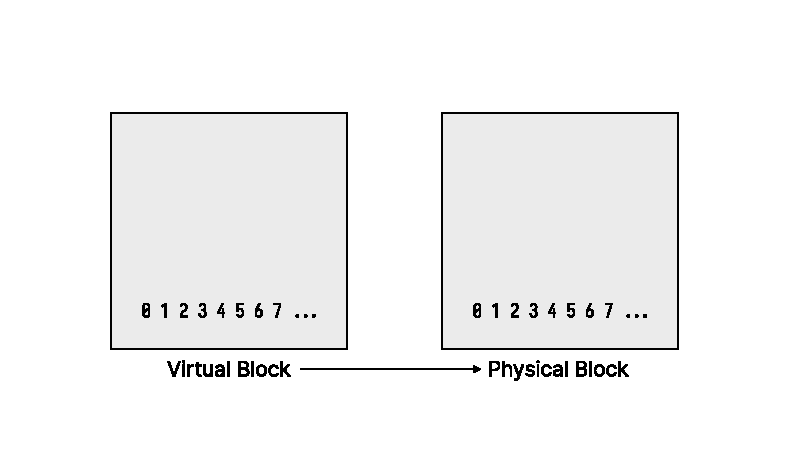
\includegraphics{virt-to-phy-block.eps}

  \end{slide}

  \begin{slide}

    \slidetitle{Memory Management Unit (MMU)}

    Maps virtual address to physical address

    \leftspace{}Also checks permissions
    \medskip

    One technique is to divide memory up into fixed-size pages (typically 4096 bytes)

    \leftspace{}A page in virtual memory is called a page

    \leftspace{}A page in physical memory is called a frame

  \end{slide}

  \begin{slide}

    \slidetitle{You Typically Do Not Use All 64 Virtual Address Bits}

    CPUs may have different levels of virtual addresses you can use

    \leftspace{}Implementation ideas are the same
    \medskip

    We'll assume a 39 bit virtual address space used by RISC-V and other
    architectures

    \leftspace{}Allows for 512 GiB of addressable memory (called Sv39)
    \medskip

    Implemented with a page table indexed by Virtual Page Number (VPN)

    \leftspace{}Looks up the Physical Page Number (PPN)

  \end{slide}

  \begin{slide}

    \slidetitle{The Page Table Translates Virtual to Physical Addresses}

    \begin{center}
      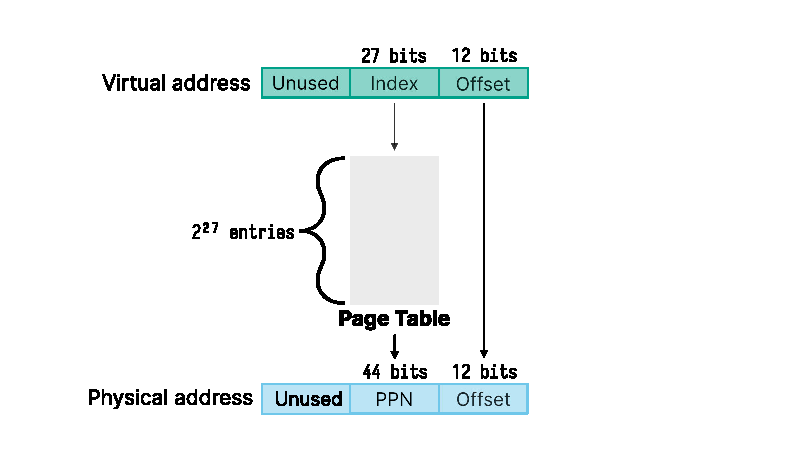
\includegraphics{single-level-page-table.eps}
    \end{center}

  \end{slide}

  \begin{slide}

    \slidetitle{The Page Table Entry (PTE) Also Stores Flags in the Lower Bits}

    \begin{center}
      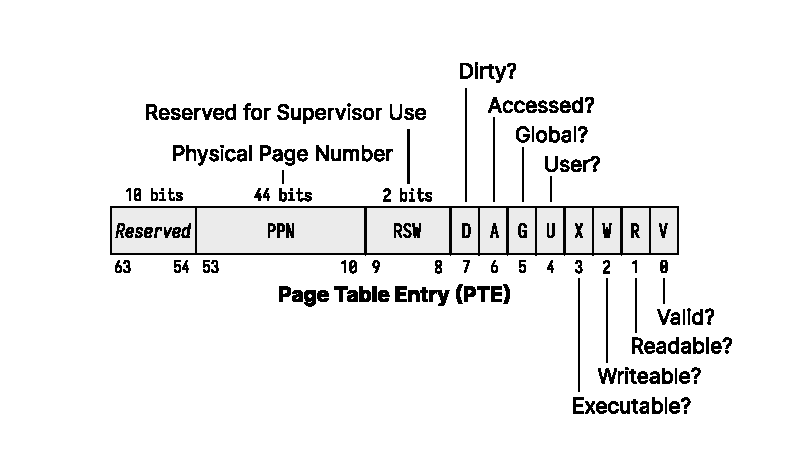
\includegraphics{pte.eps}
    \end{center}

  \end{slide}

  \begin{slide}

    \slidetitle{The Kernel Handles Translating Virtual Addresses}

    Considering the following page table:
    \begin{center}
    {\ttfamily
    \begin{tabular}{ll}
      VPN  & PPN  \\
      0x0 & 0x1 \\
      0x1 & 0x4 \\
      0x2 & 0x3 \\
      0x3 & 0x7 \\
    \end{tabular}}
    \end{center}
    \medskip

    We would get the following virtual $\rightarrow$ physical address translations:
    \begin{center}
    \texttt{0x0AB0} $\rightarrow$ \texttt{0x1AB0}

    \texttt{0x1FA0} $\rightarrow$ \texttt{0x4FA0}

    \texttt{0x2884} $\rightarrow$ \texttt{0x3884}

    \texttt{0x32D0} $\rightarrow$ \texttt{0x72D0}
    \end{center}

  \end{slide}

  \begin{slide}

    \slidetitle{Page Translation Example Problem}

    Assume you have a 8-bit virtual address, 10-bit physical address

    \leftspace{}and each page is 64 bytes
    \medskip

    \begin{itemize}
      \item How many virtual pages are there? \onslide<2->{$\mathsf{\frac{2^8}{2^6} = 4}$}
      \item How many physical pages are there? \onslide<2->{$\mathsf{\frac{2^{10}}{2^6} = 16}$}
      \item How many entries are in the page table? \onslide<2->{$\mathsf{4}$}
      \item Given the page table is \texttt{{[0x2, 0x5, 0x1, 0x8]}}

            \hspace{2em} what's the physical address of \texttt{0xF1}?

            \onslide<2->{\texttt{0x231}}
    \end{itemize}

  \end{slide}

  \begin{slide}

    \slidetitle{Each Process Gets Its Own Page Table}

    When you \texttt{fork} a process, it will copy the page table from the parent

    \leftspace{}Turn off the write permission so the kernel can implement
    copy-on-write
    \medskip

    The problem is there are $\mathsf{2^{27}}$ entries in the page table, each
    one is 8 bytes

    \leftspace{}This means the page table would be 1 GiB
    \medskip

    Note that RISC-V translates a 39-bit virtual to a 56-bit physical address

    \leftspace{}It has 10 bits to spare in the PTE and could expand

    \leftspace{}Page size is 4096 bytes (size of offset field)

  \end{slide}

  \begin{slide}

    \slidetitle{You May Be Thinking That Seems Like A Lot of Work}

    In the ``Subprocess'' lecture, we're doing a \texttt{fork} followed by
    \texttt{exec}

    \leftspace{}why do we need to copy the page tables?
    \medskip

    We don't! There's a system call for that --- \texttt{vfork}
    \medskip

    \texttt{vfork} shares all memory with the parent

    \leftspace{}It's undefined behavior to modify anything
    \medskip

    Only used in very performance sensitive programs

  \end{slide}

  \begin{slide}

    \slidetitle{We Use Pages for Memory Translation}

    Divide memory into blocks, so we only have to translate once per block
    \medskip

    Use page tables (array of PTEs) to access the PPN (and flags)
    \medskip

    New problem: these page tables are always huge!

  \end{slide}

\end{document}
